% !TEX TS-program = Xelatex
% !TEX encoding = UTF-8 Unicode

\documentclass[UTF8]{ctexart}
\usepackage{amsmath}
\usepackage[bottom]{footmisc}
\usepackage{geometry}
\usepackage{graphicx}
\usepackage{hyperref}
\usepackage{figsize}
\usepackage[separate-uncertainty = true,per-mode=symbol]{siunitx}
\usepackage{tabu}
\usepackage{wasysym}
\geometry{left=0.7in,right=0.7in,bottom=0.7in,top=0.7in}
\begin{document}

\title{实验三十:用示波器观察动态磁滞回线}
\author{朱寅杰 1600017721}
\date{2018年6月15日}
\maketitle
\setcounter{section}{30}

\subsection{铁氧体的饱和磁滞回线}
取励磁电流频率为$f=\SI{100}{\Hz}$,观察铁氧体的饱和磁滞回线。测量励磁电流所用的电阻$R_1=\SI{2.0}{\ohm}$,测量磁感应强度所用的RC电路为$R_2=\SI{50}{k\ohm}$,$C=\SI{10.0}{\micro\F}$。

磁场强度$H$由励磁电流算出:$H=U_{R_1}N_1/lR_1$。当$R_2C\gg1/f$时,磁感应强度由RC电路积分得到:$B=U_CR_2C/N_2S$。书上给出了$N_1=N_2=150$,$S=\SI{1.24e-4}{\m\squared}$,$l=\SI{.130}{\meter}$,数据如下表。
\begin{center}
\begin{tabu}{X[c,-10]X[c,-10]X[c,-10]X[c,-10]||X[c,-10]X[c,-10]X[c,-10]X[c,-10]}
\hline
$U_{R_1}$/mV&$U_C$/mV&$H$/(A/m)&$B$/T&$U_{R_1}$/mV&$U_C$/mV&$H$/(A/m)&$B$/T\\
\hline
400&	14.85&	230.77 &	0.3992 &	-400&	-14.8&	-230.77 &	-0.3978
\\300&	14.55&	173.08 &	0.3911 &	-300&	-14.6&	-173.08 &	-0.3925
\\200&	14.05&	115.38 &	0.3777 &	-200&	-14.05&	-115.38 &	-0.3777
\\150&	13.5&	86.54 &	0.3629 &	-100&	-12.75&	-57.69 &	-0.3427
\\100&	12.5&	57.69 &	0.3360 &	-50&	-10.7&	-28.85 &	-0.2876
\\80&	11.85&	46.15 &	0.3185 &	-20&	-7.45&	-11.54 &	-0.2003
\\60&	10.95&	34.62 &	0.2944 &	0&	-4.2&	0.00 &	-0.1129
\\40&	9.45&	23.08 &	0.2540 &	23.6&	0&	13.62 &	0.0000
\\20&	7&	11.54 &	0.1882 &	50&	4.4&	28.85 &	0.1183
\\0&	3.7&	0.00 &	0.0995 &	100&	10.45&	57.69 &	0.2809
\\-20.2&	0&	-11.65 &	0.0000 &	150&	12.65&	86.54 &	0.3401
\\-40&	-3.75&	-23.08 &	-0.1008 &	200&	13.6&	115.38 &	0.3656
\\-60&	-6.95&	-34.62 &	-0.1868 &	300&	14.5&	173.08 &	0.3898
\\-80&	-9.25&	-46.15 &	-0.2487 &	400&	14.9&	230.77 &	0.4005
\\-100&	-10.9&	-57.69 &	-0.2930 &	&	&	&	
\\-150&	-12.75&	-86.54 &	-0.3427 &	&	&	&	
\\-200&	-13.6&	-115.38 &	-0.3656 &	&	&	&	
\\-300&	-14.35&	-173.08 &	-0.3858 &	&	&	&	
\\-400&	-14.8&	-230.77 &	-0.3978 &	&	&	&	
\\
\hline
\end{tabu}
\end{center}
从表中读出,饱和磁感应强度$B_s=\SI{.399}{\T}$,磁场退至零时剩余磁感应强度为(取正负平均)$B_r=\SI{.106}{\T}$,矫顽力为(取正负平均)$H_c=\SI{12.635}{A/m}$。磁滞回线如下图:
\begin{figure}[h]
  \centering
  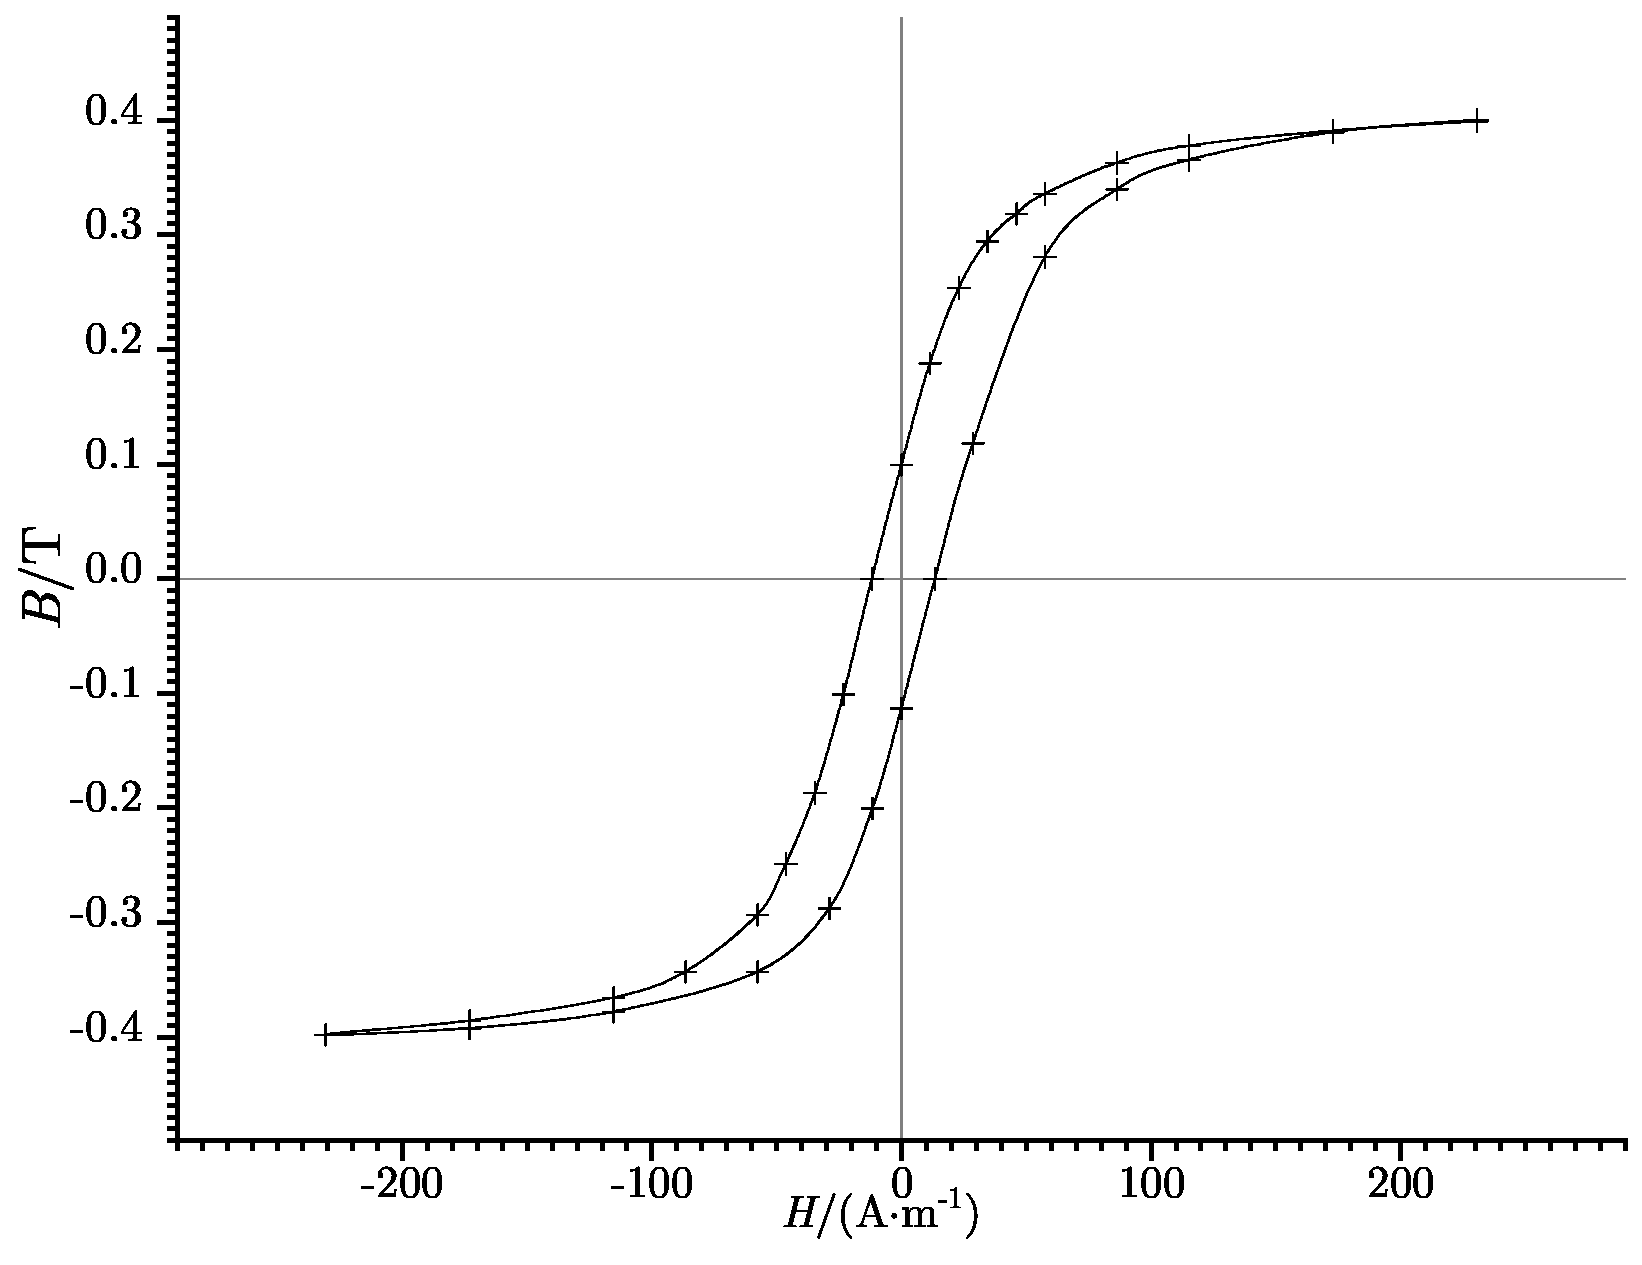
\includegraphics[width=0.5\linewidth]{B-H.eps}
  \caption{铁氧体的饱和磁滞回线。在\SI{100}{\Hz}的外场下测出}
\end{figure}

再观察不同频率下铁氧体的饱和磁滞回线:
\begin{center}
\begin{tabu}{X[c,-10]|X[c,-10]X[c,-10]X[c,-10]X[c,-10]|X[c,-10]X[c,-10]}
\hline
$f$/Hz&\multicolumn2{c}{$U_{C}^{(r)}$/mV}&\multicolumn2{c|}{$U_{R_1}^{(c)}$/mV}&$H_c$/(A/m)&$B_r$/T\\
\hline
50	&3.58	&-3.92	&-20	&21.8	&12.058 	&0.101 \\
100	&3.7	&-4.2	&-20.2	&23.6	&12.639 	&0.106 \\
150	&3.6	&-3.65	&-20.2	&20.6	&11.769 	&0.097 \\
\hline
\end{tabu}
\end{center}
可以看出在\SI{50}{\Hz}~\SI{150}{\Hz}的范围内铁氧体饱和磁滞回线的剩余磁感应强度$B_r$矫顽力$H_c$都是基本不变的。

示波器的仪器误差为测量值的2\%加上满刻度值的0.3\%,酌情再算上一个满刻度值的1\%的观测误差(光标没法完全对准)。以上述测量到$U_C^{(c)}=\SI{-20}{mV}$为例,满刻度值为\SI{50}{\mV},仪器允差为\SI{0.55}{\mV},除以根号三以后和观测误差\SI{.5}{\V}合成得到不确定度约为$\sqrt{(\SI{.55}{\mV})^2/3+(\SI{.50}{\mV})^2}=\SI{.59}{\mV}$,大约是一个3\%的误差。表中其他电压测量值的不确定度也基本是这个大小左右。$H$与$B$都是直接正比于电压,其不确定度也就约为3\%上下。
\subsection{论正确选取积分电路时间常数$R_2C$的重要性}
如果将监测磁感应强度用的$RC$积分电路的参数换掉,把$R_2C$的值改小,那么$U_C$将不能反映真实的磁感应强度值。我们保持$f=\SI{50}{\Hz}$,分别取$R_2C$为\SI{.5}{s}、\SI{.05}{s}和\SI{.01}{s},记录下屏幕上的图案:
\begin{figure}[h]
  \centering
  \subfigure[$R_2C=\SI{.5}{\s}$时的图像。此时$B$与$U_C$成正比。]{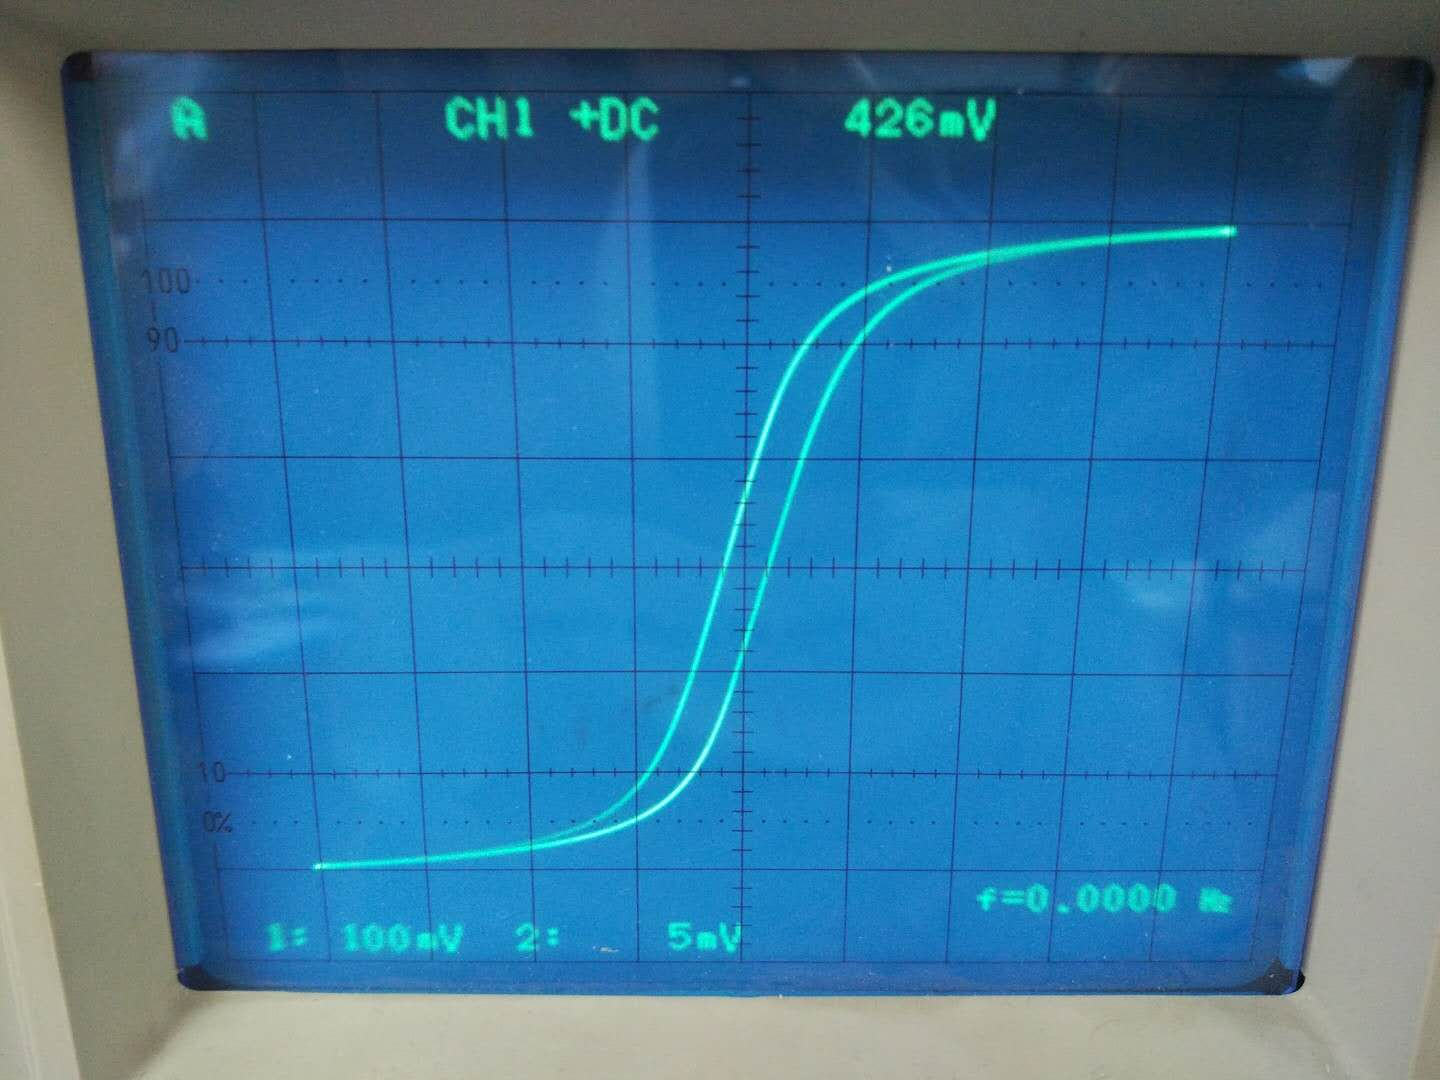
\includegraphics[width=0.3\linewidth]{5.jpg}}
  \hfill
  \subfigure[$R_2C=\SI{.05}{\s}$时的图像。此时$U_C$不再反映$B$,而是有了畸变。]{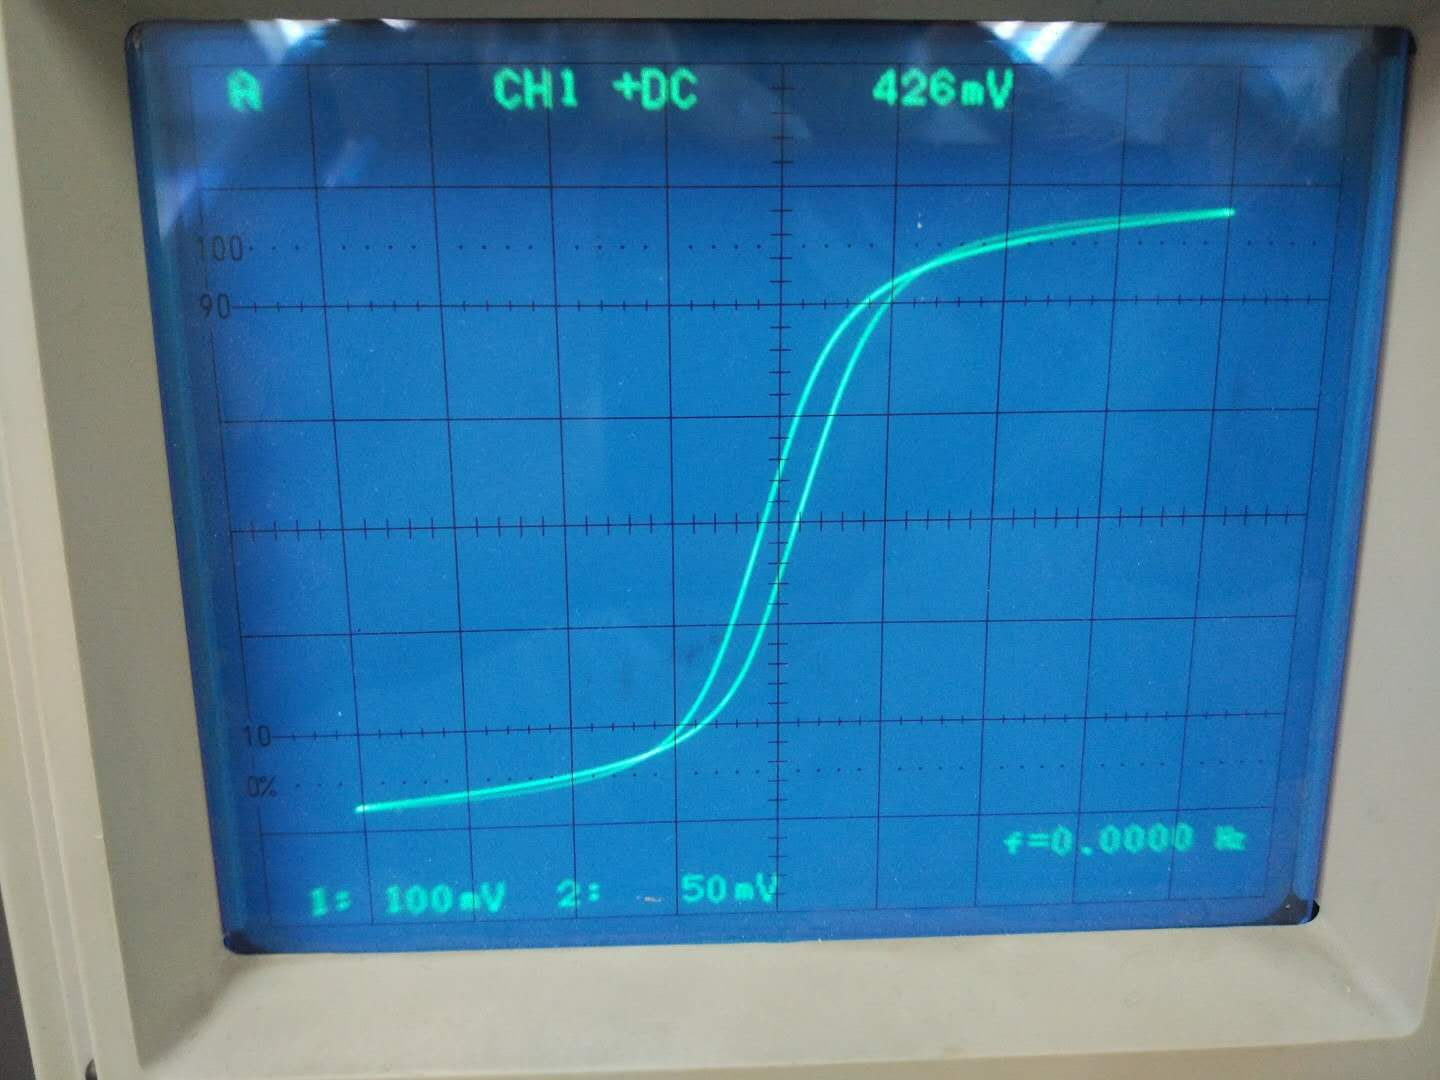
\includegraphics[width=0.3\linewidth]{05.jpg}}
  \hfill
  \subfigure[$R_2C=\SI{.01}{\s}$时的图像。此时$U_C$不再反映$B$,而是有了畸变。]{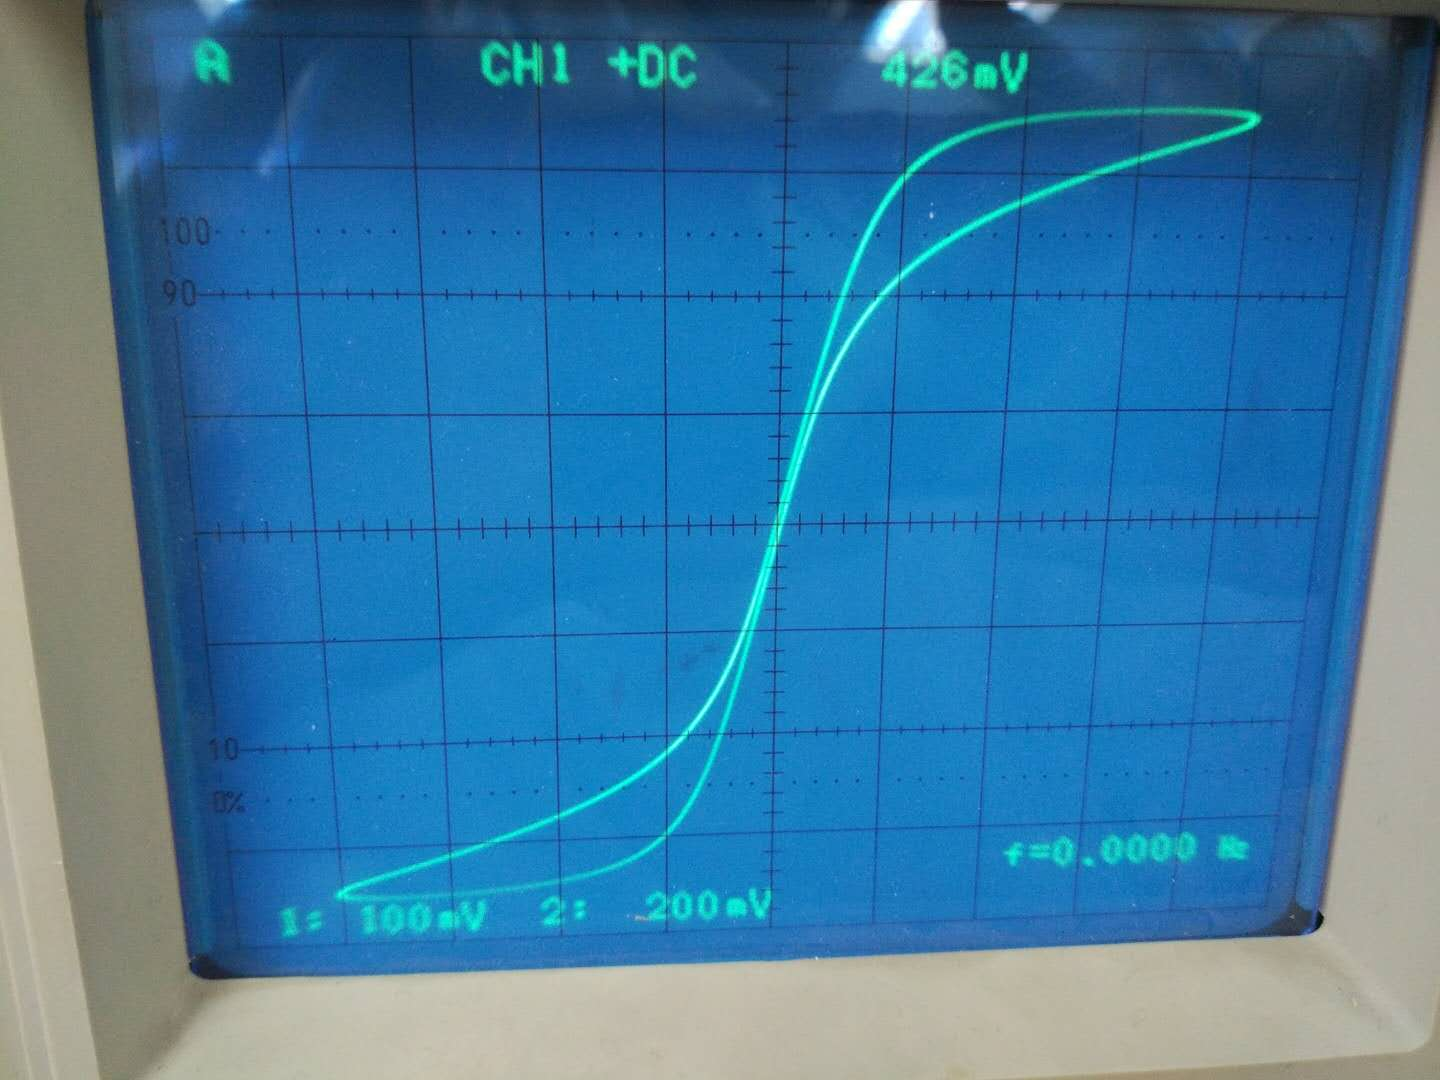
\includegraphics[width=0.3\linewidth]{01.jpg}}
  \\
\end{figure}
$R_2C=\SI{.01}{\s}$的话这个时间常量甚至小于交变场变化的周期,此时$RC$电路不再是一个好的积分电路了。
\subsection{铁氧体的动态磁化曲线}
取励磁电流频率为$f=\SI{100}{\Hz}$,观察铁氧体的动态磁滞回线。测量励磁电流所用的电阻$R_1=\SI{2.0}{\ohm}$,测量磁感应强度所用的RC电路为$R_2=\SI{50}{k\ohm}$,$C=\SI{10.0}{\micro\F}$。磁场强度$H$由励磁电流算出:$H=U_{R_1}N_1/lR_1$。当$R_2c\gg1/f$时,磁感应强度由RC电路积分得到:$B=U_CR_2C/N_2S$。再由此算出振幅磁导率$\mu_m=B_m/\mu_0H$。书上给出了$N_1=N_2=150$,$S=\SI{1.24e-4}{\m\squared}$,$l=\SI{.130}{\meter}$,数据如下表。
\begin{center}
\begin{tabu}{X[c,-10]X[c,-10]X[c,-10]X[c,-10]X[c,-10]||X[c,-10]X[c,-10]X[c,-10]X[c,-10]X[c,-10]}
\hline
$U_{R_1}^{(m)}$/mV	&$U_C^{(m)}$/mV	&$H_m$/(A/m)	&$B_m$/mT	&$\mu_m$	&$U_{R_1}^{(m)}$/mV	&$U_C^{(m)}$/mV	&$H_m$/(A/m)	&$B_m$/mT	&$\mu_m$
\\
\hline
2	&0.17 	&1.15 	&4.57 	&3151.7 	&50	&5.90 	&28.85 	&158.60 	&4375.3
\\
4	&0.32 	&2.31 	&8.60 	&2966.3 	&60	&6.84 	&34.62 	&183.87 	&4227.0
\\
6	&0.49 	&3.46 	&13.17 	&3028.1 	&80	&9.70 	&46.15 	&260.75 	&4495.8
\\
8	&0.70 	&4.62 	&18.82 	&3244.4 	&100	&10.60 	&57.69 	&284.95 	&3930.4
\\
10	&0.86 	&5.77 	&23.12 	&3188.8 	&120	&11.70 	&69.23 	&314.52 	&3615.2
\\
15	&1.36 	&8.65 	&36.56 	&3361.8 	&150	&12.65 	&86.54 	&340.05 	&3127.0
\\
20	&1.94 	&11.54 	&52.15 	&3596.7 	&168	&13.10 	&96.92 	&352.15 	&2891.3
\\
25	&2.48 	&14.42 	&66.67 	&3678.2 	&200	&13.55 	&115.38 	&364.25 	&2512.1
\\
30	&3.16 	&17.31 	&84.95 	&3905.7 	&250	&14.20 	&144.23 	&381.72 	&2106.1
\\
40	&4.38 	&23.08 	&117.74 	&4060.2 	&300	&14.55 	&173.08 	&391.13 	&1798.3
\\
\hline
\end{tabu}
\end{center}
\begin{figure}[h]
  \centering
  \subfigure[铁氧体的动态磁化曲线。]{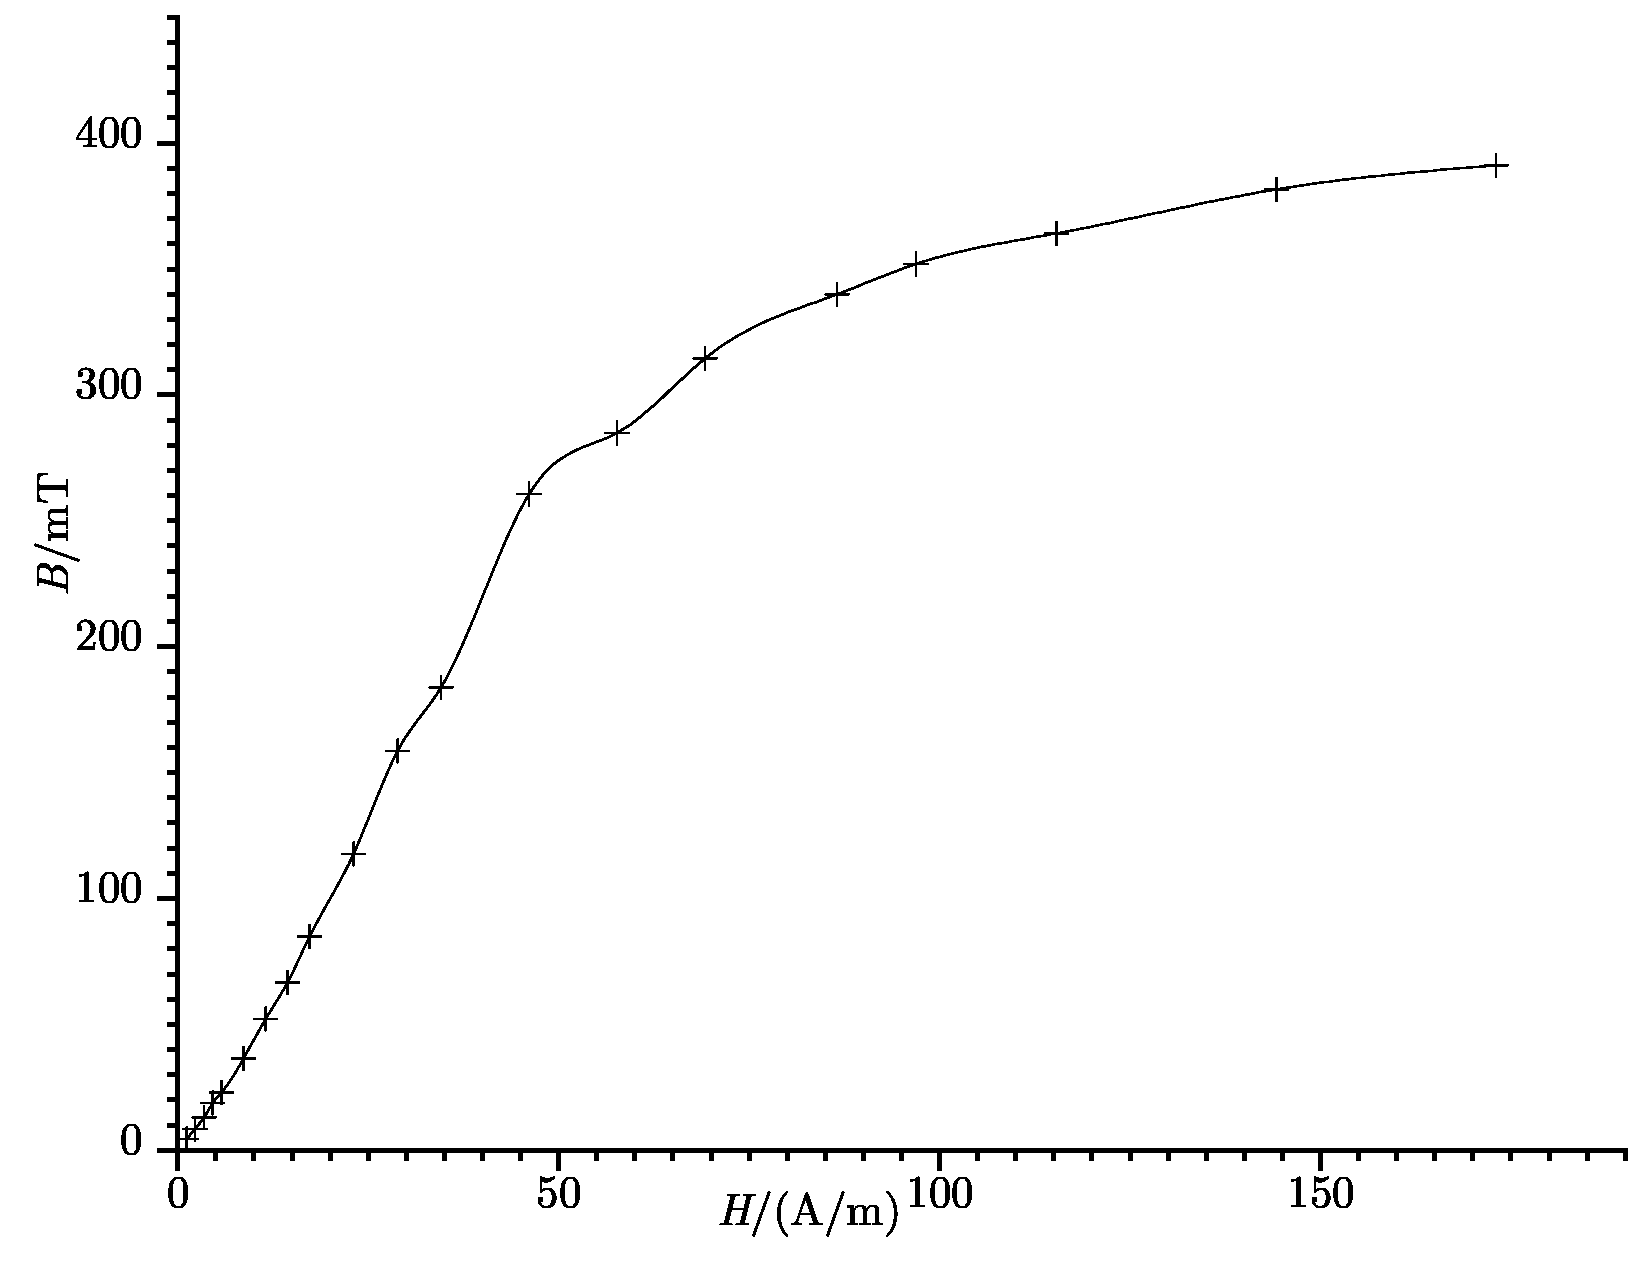
\includegraphics[width=0.49\linewidth]{dongtai.eps}}\hfill
  \subfigure[振幅磁导率$\mu_m$随磁场峰值$H_m$的变化。]{\includegraphics[width=0.49\linewidth]{mu-H.eps}}
\end{figure}
可以观察到对于铁氧体,开始时$B$随$H$增大而增大,在$H$很小时接近于正比例变化;当$H$较大时,$B$随$H$增加会越变越缓慢。振幅磁导率$\mu_m$在$H\approx0$时从一个常数出发,随着$H$的增大先达到一个峰值(不去理会有些lie out的数据点),再随$H$的增大而迅速减小。当$H\rightarrow0$时,$\mu_m$趋于一个常数,记为起始磁导率$\mu_i$。利用$U_{R_1}$在\SI{10}{\mV}以下的五个数据点作回归,从斜率算出$\mu_i=\num{3263(103)}$,相关系数为\num{.99852}。
\subsection{硅钢的磁滞回线}
取励磁电流频率分别为$f=$\SI{20}{\Hz}、\SI{40}{\Hz}、\SI{60}{\Hz}。电路中其他元件参数不变,保持$U_{R_1}^{(m)}=\SI{.4}{\V}$(相当于$H_m=\SI{400}{A\per\meter}$),调出硅钢片的磁滞回线,从示波器上读电压,计算$B_m$、$B_r$与$H_c$。硅钢磁芯$l=\SI{.075}{\m}$,$S=\SI{1.20e-4}{\m\squared}$,匝数$N=150$。结果如下表。
\begin{center}
\begin{tabu}{X[c,-10]|X[c,-10]X[c,-10]X[c,-10]|X[c,-10]X[c,-10]X[c,-10]}
\hline
$f$/Hz&$U_{C}^{(m)}$/mV&$U_{C}^{(r)}$/mV&$U_{R_1}^{(c)}$/mV&$B_m$/T&$B_r$/T&$H_C$/(A/m)\\
\hline
20	&33.6	&21.2 	&100 	&0.933 	&0.589 	&100 \\
40	&33.6	&22.4 	&117 	&0.933 	&0.622 	&117 \\
60	&33.6	&23.4 	&134 	&0.933 	&0.650 	&134 \\
\hline
\end{tabu} 
\end{center}
可以看出,硅钢动态磁滞回线中,磁感应强度的峰值$B_m$只取决于外场大小,不随频率变化;而保持外场不变时,剩余磁感应强度$B_r$与矫顽力$H_c$随频率的增加而变大,磁滞回线变得更为矮胖,围成的面积也变得更大。说明在高一些的频率的磁场中硅钢的磁滞效应更显著,能量损耗会更大。
\subsection{思考题}
动态磁滞回线是在一个给定频率的交变外磁场下材料磁化行为的曲线,曲线形状与外场的振幅与频率都可能有关,而静态磁滞回线是缓慢变化外场$H$,测一个$H$测一个$B$,完事了再测下一个$H$和$B$,$H$变化的速度很慢。铁磁材料的动态磁滞回线回收到磁场变化幅度和频率的影响。

在实验所测的\SI{100}{\Hz}以下的低频上(虽然两个材料实际测量用的频率,外场强度也不一样,但还是能做比较的。铁氧体加的外场比硅钢小,但是铁氧体在较小的外场下已经饱和,再加更大的外场并不会对$H_C$和$B_r$造成多大的改变),铁氧体的饱和剩余磁感应强度在\SI{0.1}{\T}左右,矫顽力在\SI{12}{A\per\meter}左右;硅钢的剩余磁感应强度达到\SI{.6}{\T},矫顽力在\SI{100}{\A\per\m}以上。这说明铁氧体比硅钢更接近软磁体,撤去外场以后硅钢的。同时铁氧体的矫顽力和剩余磁感应强度随频率没有显著变化,而硅钢的磁滞现象随着频率的增加会显著地变强。

要让电容上的电压正确反映磁感应强度,就要让$R_2C\gg1/f$,即$RC$积分电路的时间常数远大于磁感应强度的变化周期。

横轴为$H$纵轴为$B$的话,那磁滞回线一定是逆时针绕行的。这是因为磁滞回线围成的面积代表外磁场变化一个周期下来在铁磁体上的能量损耗,如果顺时针绕行的话就不是损耗而是凭空变出能量了,这是不可能的。
\end{document} 